\documentclass[12pt]{standalone}
\usepackage{tikz}
\usetikzlibrary{patterns} % calc, arrows.meta, decorations.pathreplacing}

\begin{document}
%\begin{figure}[t]
%	\begin{center}
		%lwarp%\begin{lateximage}[a half-open square][][width: 40\%;]
		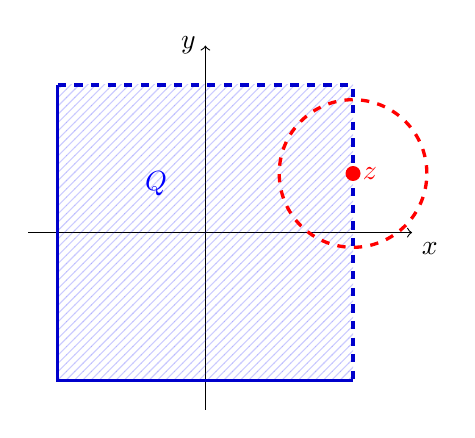
\begin{tikzpicture}[scale=1.25]
			% Axes
			\draw[->] (-1.8, 0) -- (2.1, 0) node[below right] {$x$};
			\draw[->] (0, -1.8) -- (0, 1.9) node[left] {$y$};
			% d∞-unit ball (max metric) with light blue pattern
			\fill[pattern color=blue, opacity=0.2, pattern=north east lines] (1.5, 1.5) -- (1.5, -1.5) -- (-1.5, -1.5) -- (-1.5, 1.5) -- cycle;
			
			% Outline
			\draw[black!20!blue, very thick, dashed] (-1.5, 1.5) -- (1.5, 1.5) -- (1.5, -1.5);
			\draw[black!20!blue, very thick] (-1.5,1.5) -- (-1.5,-1.5) -- (1.5, -1.5);
			
			\filldraw[red] (1.5, 0.6) circle (2pt) node[anchor=west] {$z$};
			\draw[red, dashed, very thick] (1.5,0.6) circle (0.75);
			\node[blue] at (-0.5,0.5) {$Q$};
		\end{tikzpicture}	
		%lwarp%\end{lateximage}
%	\end{center}
%	\caption{\textit{$Q$ is the half-open square $\{-1\le x<1$, $-1\le y<1\}$; $z\notin Q$ but $z\in\overline Q$}}
%	\label{fig:halfopensquare}
%\end{figure}
\end{document}
